\section{Data Reduction Cook-Book}
\label{sec:cookbook}

%\red{\textit{Cookbook-like description of pipeline recipes and their usage}}

\subsection{Getting Started with \esorex{}}
\label{sec:esorex-quick}

\textit{\esorex{}} is a command-line tool which can be used to execute the
recipes of all standard VLT/VLTI instrument pipelines. With \textit{\esorex{}}
in your path, the general structure of an \textit{\esorex{}} 
command line is

\begin{shell}[fontsize=\small]
%prompt esorex [esorex options] [recipe [recipe options] [sof [sof]...]]
\end{shell}

where options appearing before the recipe name are options for
\textit{\esorex{}} itself, and options given after the recipe name are options
which affect the recipe. 

All available \textit{\esorex{}} options can be listed with the command
\begin{shell}[fontsize=\small]
%prompt esorex --help
\end{shell}

and the full list of available parameters of a specific recipe can be obtained
with the command 

\begin{shell}[fontsize=\small]
%prompt esorex --help <recipe name>
\end{shell}
The output of this command shows as parameter values the current setting, \ie
all modifications from a configuration file or the command line are already
applied.

The listing of all recipes known to \textit{\esorex{}} can be obtained with the command
\begin{shell}[fontsize=\small]
%prompt esorex --recipes
\end{shell}

The last arguments of an \textit{\esorex{}} command are the so-called
\textit{set-of-frames}. A \textit{set-of-frames} is a simple text file which
contains a list of input data files for the recipe. Each input file is
followed by an unique identifier (frame classification or frame tag),
indicating the contents of this file. The input files can be given as 
absolute or relative path, and \textit{\esorex{}} allows the use of environment variables so
that a common directory prefix can be abreviated. Individual lines may be
commented out by putting the hash character (\texttt{\#}) in the first
column. An example of a \textit{set-of-frames} is shown in the following:

\begin{shell}[fontsize=\small]
%prompt cat darks.sof
/data/crires/CRIRES.2019-03-29T09:50:36.645.fits DARK
$RAW_DATA/CRIRES.2019-03-29T09:52:16.513.fits DARK
$RAW_DATA/CRIRES.2019-03-29T09:53:47.996.fits DARK
#$RAW_DATA/CRIRES.2019-03-29T09:55:04.515.fits DARK
#$RAW_DATA/dark5.fits DARK
\end{shell}

These \textit{set-of-frames} files will have to be created by the user using a
text editor, for instance.

Finally, if more than one \textit{set-of-frames} is given on the command-line
\textit{\esorex{}} concatenates them into a single \textit{set-of-frames}.


\subsection{Calibration, made easy}
\label{sec:simcalexpl}
This example follows the data flow described in \ref{sec:simplecalib}. It makes
use of a pre-existing TW-table, for example the one from the CalibDB, for order
traces and slit-tilt. All data needs to match in spectrograph setting.

\texttt{cr2res\_cal\_dark} only receives raw frames, so the SOF looks like the
one just above and gets processed like
\begin{shell}[fontsize=\small]
  %prompt esorex cr2res_cal_dark darks.sof
\end{shell}  
The outputs are master darks and BPM. The recipe parameters influence how
outliers are rejected and where to put the threshold for rejecting pixels as
bad. The default values should give good results.

Next are the FLATs.
\begin{shell}[fontsize=\small]
%prompt cat flats.sof
$RAW/flat1.fits         FLAT
$RAW/flat2.fits         FLAT
$RAW/flat3.fits         FLAT
$CALIB/dark_bpm.fits    CAL_DARK_BPM
$CALIB/dark_master.fits CAL_DARK_MASTER
$CALIB/tw.fits          UTIL_WAVE_TW
cr2res_detlin_coeffs.fits  CAL_DETLIN_COEFFS

%prompt esorex cr2res_cal_flat flats.sof
\end{shell}
The main data product is the normalized flat-field
(\verb!PRO.CATG=CAL_FLAT_MASTER!). Note that even though the recipe can perform
the order-tracting by itself, it is recommended to provide a TW as input;
especially in the bands YJHK, where the slit-tilt can be characterized. This way
absorption lines affect the flat-field less.


For wavelength-calibration, both the UNE and FPET frames should best be provided
at once:
\begin{shell}[fontsize=\small]
%prompt cat wave.sof
$RAW/une.fits           WAVE_UNE
$RAW/fpet.fits          WAVE_FPET
$CALIB/dark_bpm.fits    CAL_DARK_BPM
$CALIB/dark_2s_master.fits CAL_DARK_MASTER
$CALIB/tw.fits          UTIL_WAVE_TW
$CALIB/cr2res_detlin_coeffs.fits  CAL_DETLIN_COEFFS

%prompt esorex cr2res_cal_wave wave.sof
\end{shell}
This produces a new TW, with updated wavelength solutions and retaining information like the order traces from the input TW.

In this simplified reduction, we rely on a pre-existing TW for traces and slit-tilt, and pre-made non-linearity correction. This normally should not negatively impact the quality of the data products, especially when metrology is used to increase the repeatability of the instrument.

%%%%%%%%%%%%%%%%%%
%%%%%%%%%%%%%%%%%%
\subsection{Examples of science reductions}

\subsubsection{Nodding}
\label{sec:nodding}
An example SOF and esorex-call for \verb!cr2res_obs_nodding! were already shown
in Ch.~\ref{sec:sci-reduc} and there really is not much more to it. Note that
there is no master-dark provided, and indeed it is not recommended doing so,
because it likely worsens the results compared to relying on the subtraction of
A and B frames from each other for removing detector features and background.

An aspect to consider is how much of an observed nodding sequence is given to
the recipe at a time. It will combine all the A-frames and all B-frames (saved
as \verb!PRO.CATG=OBS_NODDING_COMBINED[AB]!), then do the pair-wise subtraction
and spectrum extraction, resulting in a single set of spectra (from all
detector-orders) for A, and one for B (\verb!OBS_NODDING_EXTRACT[AB]!).
Therefore, if time-evolution plays a role in the science, a set of data might
need to be split up and reduced individually. An equal number of frames for
positions A and B always needs to be supplied.

The recipe also produces spectra that are combined from A and B
(\verb!OBS_NODDING_EXTRACT_COMB!). This naturally involves resampling and
relying on the wavelength scale, because the tilted slit makes the spectral
binning different between the top and bottom halves of the slit. This is why the
spectra \emph{before} this combination are considered the primary data product.
The combined spectrum contains the summed ADUs from A and B.

The jitter around positions A and B does not need to be treated explicitly by
the DRS. Instead, it makes use of the fact that the extraction algorithm
(cf.~\ref{sec:extract}) can handle arbitrary slit-illumination functions, in
this case the combined frame simply looks like multiple "stars" along the slit.

A few parameters can be tweaked to potentially improve results. If there remain
detector features that correlate with the detector columns in the combined
frames, as has sometimes been found to be the case,
\verb!--subtract_nolight_rows! can be set to \verb!TRUE!. This makes use of the
bottom 40 rows of the detectors which are intentionally baffled to not receive
light. A vertical median over these rows is calculated, and the result subtracted
from the image row-by-row.

The oversampling of the slit-function can be changed via
\verb!--extract_oversample!. This affects linearly the calculation effort of the
extraction, which in turn is the bulk of the total recipe runtime, so that
increasing the oversampling from a factor of 5 to 10 means the reduction takes
twice as long. In general, values below 5 give suboptimal results and values
above 10 are appropriate when the slit-illumination changes sharply. See
Ch.~\ref{sec:extract} for more details.

In addition to the aforementioned data products, the recipe also saves two new
TW tables with \linebreak\verb!PRO.CATG=OBS_NODDING_TW[AB]!. These correspond to
the lower and upper halves of the slit, i.e. the A and B nodding positions, and
thus have their respective slit-fractions set to \verb![0.0, 0.25, 0.5]! and
\verb![0.0, 0.75, 1.0]!. They can come handy, for example, to re-run the
extraction of a \verb!OBS_NODDING_COMBINED[AB]! frame, using
\verb!cr2res_util_extract!; or to over-plot the traces on the combined frame to
check the alignment of the target.

\subsubsection{Extracting multiple sources in nodding}
\label{sec:slitfracbinary}
In the case when multiple targets are placed on the slit (e.g resolved binary
stars) in nodding observations, a few simple steps are needed to extract the spectrum 
of each target separately. In the remainder of this section, we assume the user 
wishes to extract the spectra of two stars on the slit. The procedure can be 
adapted to handle any number of extractions.
 
Run the \verb!cr2res_obs_nodding! recipe with the default slit height.
This step is detailed in Ch.~\ref{sec:nodding} and an example SOF file is
shown in Ch.~\ref{sec:sci-reduc}.
From this step, we can disregard the extracted spectrum (as the recipe extracts
a single spectrum for the entire slit). However, we will use the combined
pair-wise subtracted A and B frames (\verb!PRO.CATG=OBS_NODDING_COMBINED[AB]!)
 illustrated in Fig.~\ref{fig:binary-nodding}.

\begin{shell}[fontsize=\small]
    %prompt esorex cr2res_obs_nodding nodd.sof
\end{shell}

\begin{figure}[!h]
  \begin{center}
    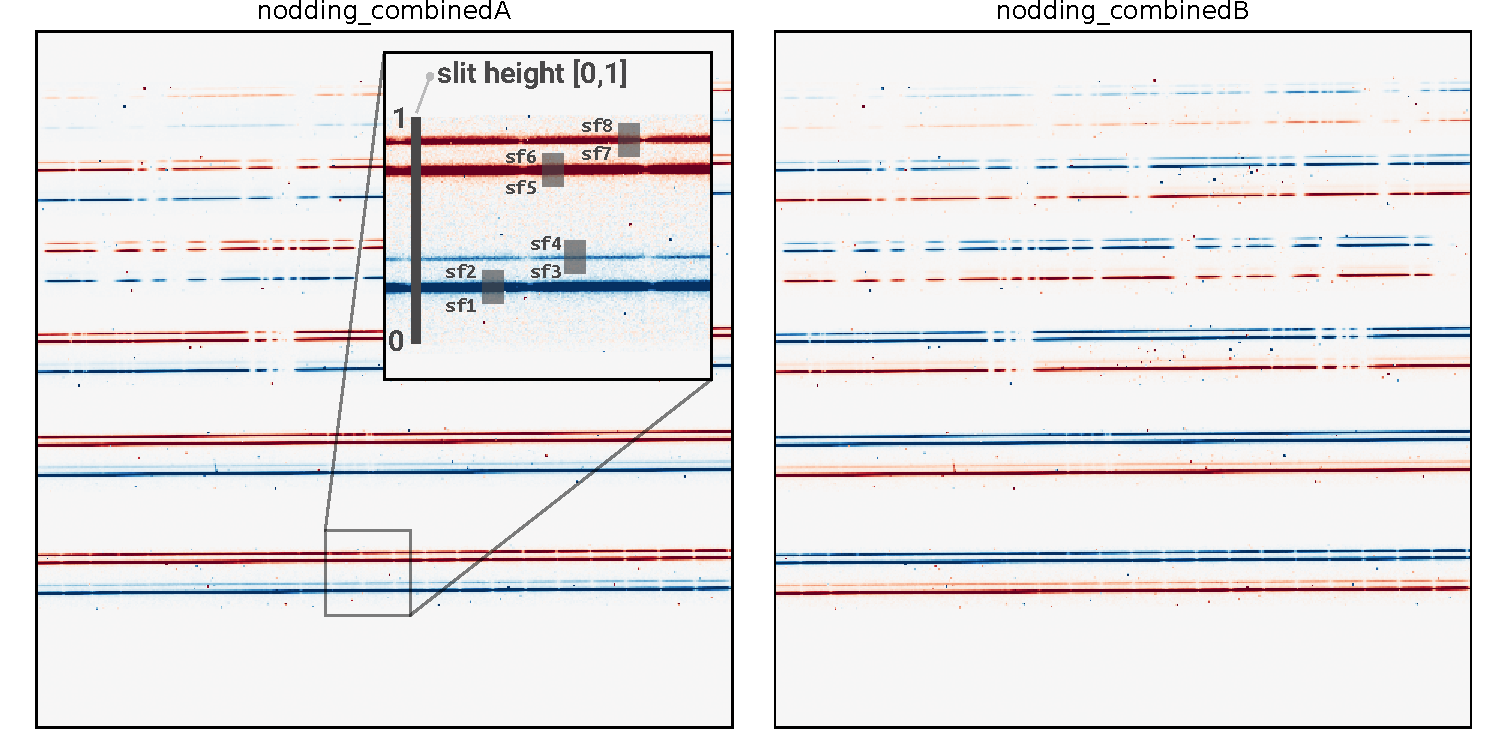
\includegraphics[width=1\textwidth]{figures/binary-nodding-combined}
  \end{center}
  \caption{
    \label{fig:binary-nodding}
    The two plots show the combinedA and combinedB frames
    on one detector. The inset on the left subplot zooms on a part of a
    spectral order, indicating the full slit height, 
    and illustrating slit fraction values to extract the spectra.}
\end{figure}

Extract the spectra of the two stars from the nodding position A -
hereafter named A1 and A2. This is done by running the \verb!cr2res_util_extract!
recipe on the combinedA frame twice, specifying slit fraction values adequate
for each of the two spectra, as illustrated in Fig.~\ref{fig:binary-nodding}.

Repeat the previous step on the combinedB frame to extract the spectra
B1 and B2, specifying adequate slit fractions.

\begin{shell}[fontsize=\small]
    %prompt mkdir A1 A2 B1 B1 # create directories to store spectra
    %prompt esorex --output-dir=A1 cr2res_util_extract --slit_frac=0.23,0.30 A.sof
    %prompt esorex --output-dir=A2 cr2res_util_extract --slit_frac=0.35,0.45 A.sof
    %prompt esorex --output-dir=B1 cr2res_util_extract --slit_frac=0.74,0.84 B.sof
    %prompt esorex --output-dir=B2 cr2res_util_extract --slit_frac=0.86,0.97 B.sof 
\end{shell}

The values of the slit-fraction listed here match the example from the figure;
they need to be adapted for each observation! The range of \verb![0.0 ... 1.0]!
corresponds to the [bottom ... top] edge 

The SOF files \verb!A.sof! and \verb!B.sof! contain only the TW file and
\begin{shell}[fontsize=\small]
    cr2res_obs_nodding_combinedA.fits OBS_NODDING_OTHER
\end{shell}
for \verb!A.sof!, and the equivalent combinedB frame for \verb!B.sof!.
No calibrations needed, because they are already applied to the combined frame.

If the user wants a single spectrum from nodding position A and for each of the
star, they still need to combine the A and B spectra -- essentially interpolating
one to the wavelength scales of the other.

\subsubsection{Staring}

\verb!cr2res_obs_staring! is very similar to \verb!cr2res_obs_nodding!, except
the nodding part. Thus, a master-dark should be supplied in the SOF, in addition
to the other files:
\begin{shell}[fontsize=\small]
%prompt cat stare.sof
$RAW/stare_exp1.fits        OBS_STARING_JITTER
$RAW/stare_exp2.fits        OBS_STARING_JITTER
$RAW/stare_exp3.fits        OBS_STARING_JITTER
$RAW/stare_exp4.fits        OBS_STARING_JITTER
$RAW/stare_exp5.fits        OBS_STARING_JITTER
$CALIB/K2192_masterflat.fits                  CAL_MASTER_FLAT
$CALIB/K2192_tw.fits                          UTIL_WAVE_TW
$CALIB/cr2res_cal_dark_K2192_bpm.fits         CAL_DARK_BPM
$CALIB/cr2res_cal_dark_K2192_30s_master.fits  CAL_DARK_MASTER
$CALIB/cr2res_detlin_coeffs.fits              CAL_DETLIN_COEFFS
\end{shell}  
Ideally, the DARK frames should match the DIT of the science frames.

If the target is always close to the center of the slit, one can decrease the extraction height for speedup.
\begin{shell}[fontsize=\small]
  %prompt esorex --extract_height=50 cr2res_obs_staring stare.sof
\end{shell}  

Analogous to the example of the binary star above, the option \verb!--slit_frac!
can be used to extract only a portion of the slit. This is useful to extract the
target and an empty portion of the slit, in order to perform sky-subtraction as
part of the analysis. Note that, due to the slit-tilt, the wavelength bins will
differ slightly between the spectra, so one needs to be resampled to the other.

\subsubsection{Generic Offset}

For data taken with the generic-offset-template, the DRS assumes that the
spatial resolution along the slit holds valuable information, and therefore does
not collapse the data into 1D-spectra. Instead, the recipe \verb!cr2res_obs_2d!
produces output tables with 2D spectra, where each in-order and not-bad pixel
has an entry with the following values and column names (prefixed with order and
trace number as for 1D spectra).

\begin{itemize}
    \item \verb!POSITIONX!, the original X-coordinate of the pixel
    \item \verb!POSITIONY!, same for Y
    \item \verb!SLIT_FRACTION!, from $[0..1]$, the spatial coordinate along the slit, i.e.~on sky.
    \item \verb!WL!, the wavelength
    \item \verb!SPEC!, the spectrum in ADU
    \item \verb!ERR!, the error spectrum.
\end{itemize}

Plotting the against wavelength and slit-fraction as X,Y-coordinates yields a
rectified 2D spectrum. Resampling to a regular grid is left to users.


The recipe interface of \verb!cr2res_obs_2d!, and thus the SOF files, follows
the same philosophy as the other \verb!cr2res_obs_*! recipes. The same processed
calibrations are listed together with the to-be-reduced raw frames.


The sky-pointings are subtracted from the object-pointings like this:

\begin{verbatim}
    if Number of SKY == Number of OBJ
         Loop on OBJ frames
             Subtract the corresponding SKY (same position in the list),
               applying the DIT correction ratio.
             Execute 2D-extraction
    else
         Average the SKY frames (if any)
         Loop in OBJ frames
             Subtract the Averaged Sky (if any) regardless of the DIT
             Execute 2D-extraction
\end{verbatim}         

\subsubsection{Polarimetry}

In polarimetry, the spectropolarimetry unit is inserted into the light path
ahead of the slit. It splits the incoming light beam into two parallel beams
of orthogonal polarization state, which then pass through a slit mask (also 
called deckers). There are two deckers: one lets the light through the first
and third quarter of the slit (each of them is 2.5" high), the other one
through the second and fourth quarter (cf.~RD01\cite{CIRESMAN}).
These two deckers are designed to cover two nodding positions, and the recipe
\verb!cr2res_obs_pol! is used in a completely analogous way to the nodding-recipe.

The SOF therefore looks just like the example from \ref{sec:sci-reduc}, except
that the raw frames are tagged \linebreak\verb!OBS_POLARIMETRY_OTHER! instead.
In addition, the recipe expects the number of raw frames to be a multiple of
$8$. This is because the observing template always takes $4$ exposures at each
nodding position, with alternating rotations of the internal optical elements;
and because the number of AB-cycles is expected to be $>0$, for background
subtraction.

As usual, the provided master calibrations are applied first. 
For the reduction of position A, the four frames from B are averaged and
subtracted, and vice versa. This works because the deckers block the light in
the respective opposite quarters of the slit.

Then the two beams are extracted from each frame, using order traces for each
decker hole. This means more extractions than for non-polarimetric observations
which is why this recipe takes significantly longer to run.

The individual extracted spectra are then combined with each other, following
the demodulation scheme described by \cite{1997MNRAS.291..658D}. The
demodulation scheme minimizes instrumental effects and produces the following
results, saved in a FITS table that is analogous to non-polarized spectra:

\begin{itemize}
    \item Intensity spectrum, i.e.~the sum of all the beams. Table columns named like \verb!i_INTENS! where \verb!i! is the order number.
    \item The Stokes parameter spectrum, i.e.~\textit{V}, \textit{Q} or \textit{U}, normalized by the intensity spectrum. These are stored in the columns \verb!i_STOKES!. Which of the Stokes parameters was observed in a dataset should be clear from your data organization, but can also be seen from the header \verb!INS.POL.TYPE!.
    \item The Null spectrum normalized by the intensity spectrum. This is a diagnostic spectrum from the demodulation that characterizes the level of spurious polarization. In the ideal case, there should be no polarization signatures present in the Null spectrum. \verb!i_NULL!.
    \item Error spectra for each of the above, in columns named like these, plus the suffix \verb!_ERR!.
    \item The array of wavelengths for each of the spectral bins.
\end{itemize}

By default, \verb!cr2res_obs_pol! does not produce intermediate outputs like the
calibrated raw frames and the decker-traces for extraction. The recipe parameter
\verb!--save_group=1! can be used to save these for a single group of $8$ raw
files, the first group in this case. Using this option results in $40$
additional files that hold the calibrated and nodding-sutracted frames, the TWs,
and the extracted spectra before demodulation.

\subsubsection{Spectro-Astrometry}

Spectro-astrometry uses the instrument derotator to take spectra with different
position angles of the slit on the sky.

The recipe \verb!cr2res_obs_nodding! can get raw input tagged like
\verb!OBS_ASTROMETRY_OTHER! or \linebreak\verb!OBS_ASTROMETRY_JITTER!. Given a sequence of
these, it will separate them by position angle and reduce the set for each angle
separately, just like plain nodding observations, with the same outputs. Any
further steps are considered out of scope for the DRS and left to users.

\subsection{Optional Steps}

\subsubsection{Throughput from standard stars}
\label{sec:throughput}
The pipeline comes with a fixed list of spectrophotometric standard stars. When \texttt{cr2res\_obs\_nodding} checks the
on-sky coordinates of the currently reduced target, and if they match one of those stars, it compares the reduced spectrum to the 
reference. The resulting throughput gets saved into a separate
data product (PRO.CATG=OBS\_NODDING\_THROUGHPUT).

Note however, that absolute flux calibration is generally not 
possible with \instrument\ because of varying slit-losses.


\subsubsection{Refining the BPM}
\label{sec:bpmrefine}
Using only the BPM that comes from \texttt{cr2res\_cal\_dark} usually gives
satisfactory results. However, pixels can be marked as bad also by being
outliers in their non-linearity behavior, or in their overall sensitivity, i.e.
in the normalized flat-field. The respective recipes each produce a BPM, and
have parameters for the thresholds.

The recipe \texttt{cr2res\_util\_bpm\_merge} allows you to merge these BPMs into
a combined BPM; \linebreak\texttt{cr2res\_util\_bpm\_split} does the inverse,
that is splitting a BPM into its original components. This is possible because
these recipes keep track of why a pixel was marked as bad. When a BPM is then
used in subsequent reduction steps, any kind of bad pixel gets masked and does
not contribute to the result.

Note that BPMs are not checked to match in spectrograph setting, so that it is
possible to use a BPM from a one setting with data from another. The same is
true for DIT.

Experience has shown that the pair-wise subtraction via nodding makes many
pixels usable that were flagged as bad pixels from the DARK frames. It can
therefore make sense, especially for low S/N spectra, to use the BPM from from
\texttt{cr2res\_cal\_flat} instead (\verb!PRO.CATG=CAL_FLAT_BPM!). To do this,
one needs to
\begin{itemize}
    \item set the \verb!--bpm_kappa! for \texttt{cr2res\_cal\_dark} to a large value (e.g. 1000) to get a master dark without pixels marked as bad. This is because otherwise the flat-field would inherit the BPM from the master dark.
    \item adjust the parameters \verb!--bpm_low! and \verb!--bpm_high! for \texttt{cr2res\_cal\_flat} to appropriate relative sensitivity thresholds.
    \item use the \verb!CAL_FLAT_BPM! in subsequent reduction steps.
\end{itemize}

\subsubsection{Splicing and Continuum Normalization}

Give extracted spectra, blaze functions and TWs from several settings to
\texttt{cr2res\_util\_splice} and it will divide by the blaze, and resample the
overlap regions between all spectra from individual detector-orders onto a
common wavelength scale, in order to then combine them with a weighted average.
The result is a single spectrum, continuous over the regions covered by the
inputs.

\begin{figure}[!h]
  \begin{center}
    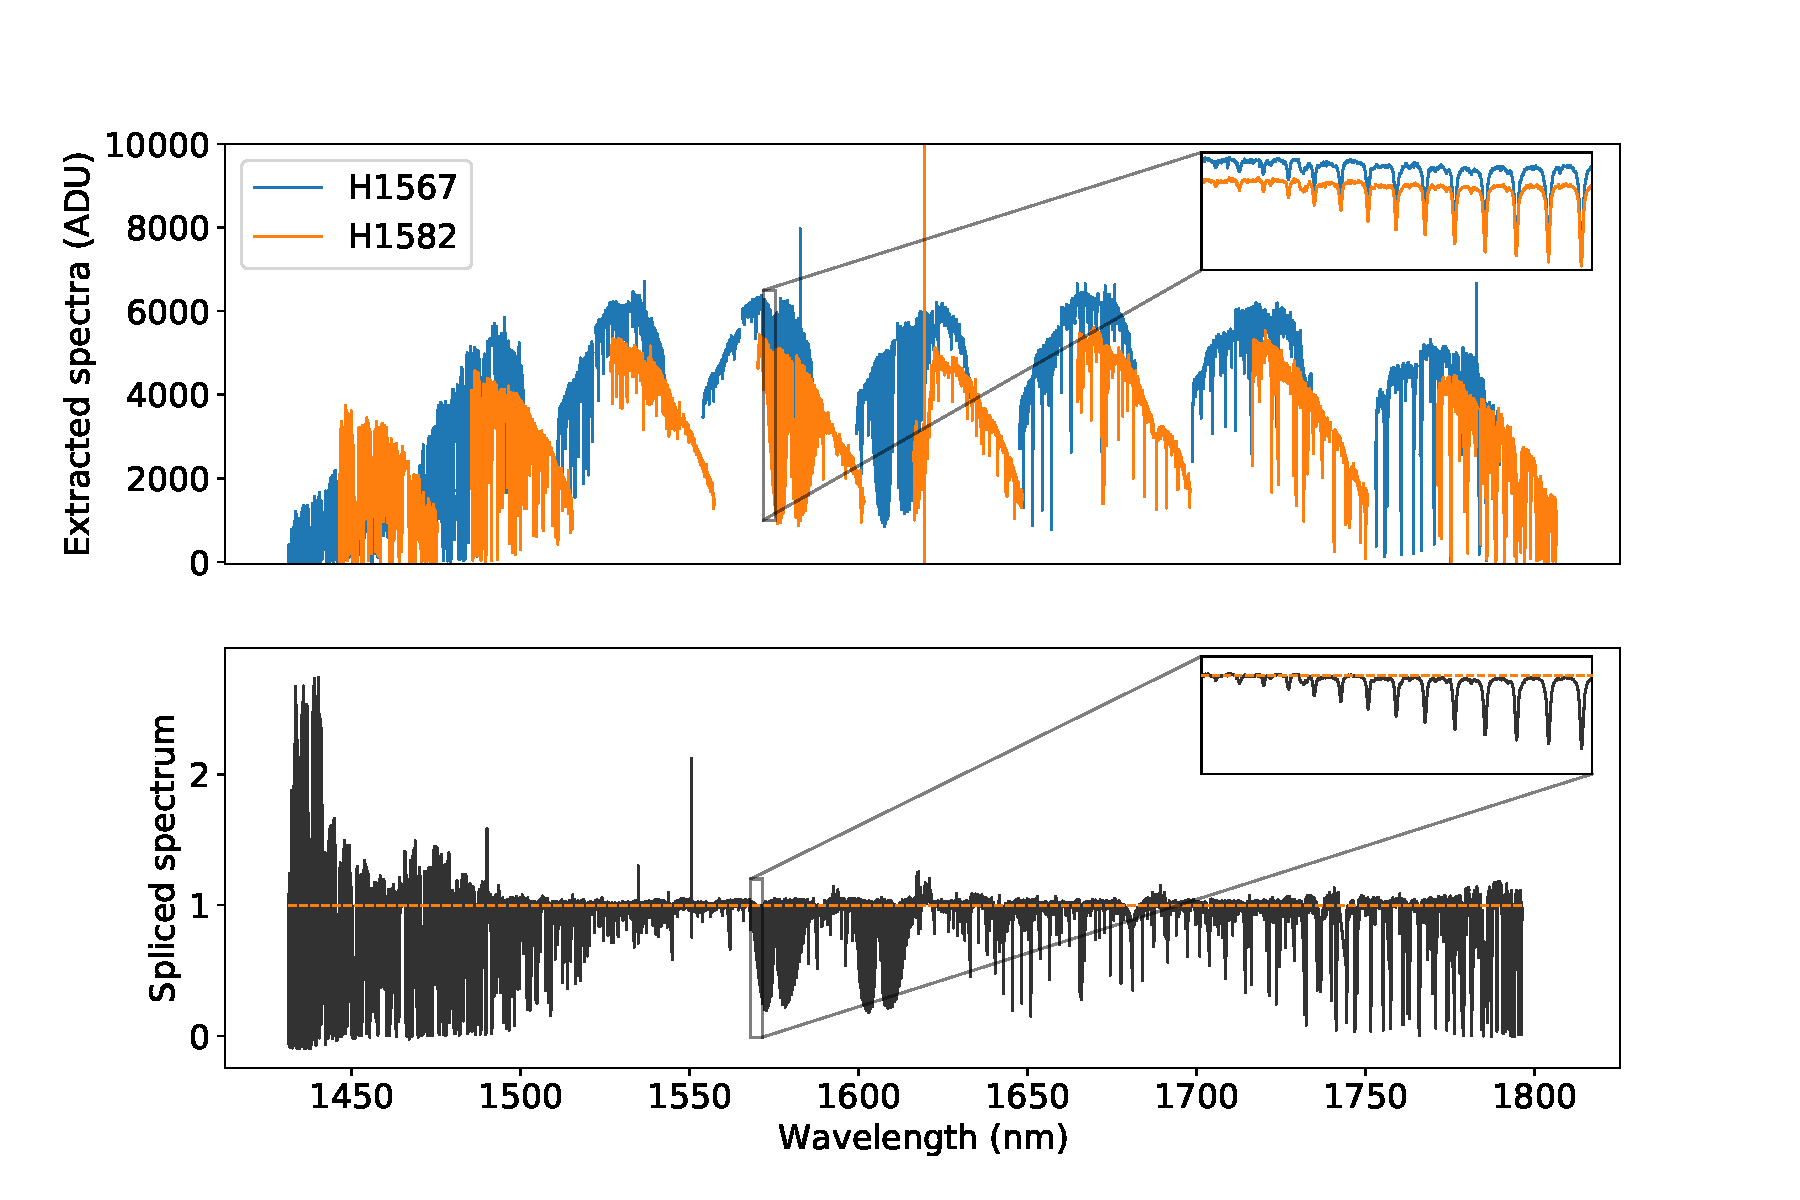
\includegraphics[width=1\textwidth]{figures/util_splice}
  \end{center}
  \caption{
    \label{fig:util_splice}
    The top subplot shows extracted spectra in two overlapping
    wavelength settings: H1567 and H1582 with an inset zoom to a narrow
    wavelength region. The bottom subplot shows the output of the splicing
    recipe. Notice that the normalization is far from perfect.}
\end{figure}

Please note that this recipe has not been tested extensively to produce reliable
results in all cases. For now its data products should therefore be considered
experimental and quality not ensured to be "science-ready". Fig.~\ref{fig:util_splice}
shows a typical example of what can be achieved with this recipe. An example SOF
file is printed below.

\begin{shell}[fontsize=\small]
%prompt cat splice.sof
H1567-cr2res_obs_nodding_extracted_combined.fits UTIL_EXTRACT_1D
H1582-cr2res_obs_nodding_extracted_combined.fits UTIL_EXTRACT_1D
$CALIB/H1567_tw.fits UTIL_WAVE_TW
$CALIB/H1582_tw.fits UTIL_WAVE_TW
$CALIB/H1567/05_cr2res_util_extract_out/
  cr2res_util_calib_calibrated_collapsed_extr1D.fits CAL_FLAT_EXTRACT_1D
$CALIB/H1582/05_cr2res_util_extract_out/
  cr2res_util_calib_calibrated_collapsed_extr1D.fits CAL_FLAT_EXTRACT_1D
\end{shell}

It should also be noted that it is probably a good idea to manually mask some
regions, like the ones affected by the ghosts, before splicing, since otherwise
this wavelength region would be degraded in the output, even if it was
unaffected in data from a different setting. 

\subsection{Calibration, from scratch}
\label{sec:calibscratch}
Following the steps outlined in Ch.~\ref{sec:stepcalib} and accompanying text,
we can reduce the calibrations without relying on pre-existing reduction
products like the TW. This is also the way the static calibrations are
assembled. The following gives example SOFs and recipe calls to reduce a single
setting.

First the SOFs:
\begin{shell}[fontsize=\footnotesize]
%prompt cat 01_cr2res_cal_dark.sof
CRIRE.2021-09-16T20:58:23.580.fits      DARK     
CRIRE.2021-09-16T20:58:40.524.fits      DARK     
CRIRE.2021-09-16T20:58:57.146.fits      DARK     
CRIRE.2021-09-16T20:59:13.835.fits      DARK     
CRIRE.2021-09-16T20:59:30.110.fits      DARK     
CRIRE.2021-09-16T20:59:46.468.fits      DARK     
CRIRE.2021-09-16T21:00:08.583.fits      DARK     
CRIRE.2021-09-16T21:02:14.863.fits      DARK     
CRIRE.2021-09-16T21:04:21.006.fits      DARK     
CRIRE.2021-09-16T21:06:27.987.fits      DARK     
CRIRE.2021-09-16T21:06:54.976.fits      DARK     
CRIRE.2021-09-16T21:07:21.609.fits      DARK     
CRIRE.2021-09-16T21:07:48.034.fits      DARK     
CRIRE.2021-09-16T21:07:57.532.fits      DARK     
CRIRE.2021-09-16T21:08:06.919.fits      DARK     

%prompt cat 02_cr2res_util_calib.sof
../cr2res_cal_detlin_coeffs.fits CAL_DETLIN_COEFFS
CRIRE.2021-09-16T20:49:23.778.fits      FLAT     
01_cr2res_cal_dark_out/cr2res_cal_dark_Y1028_3_bpm.fits CAL_DARK_BPM
01_cr2res_cal_dark_out/cr2res_cal_dark_Y1028_3_master.fits CAL_DARK_MASTER

%prompt cat 03_cr2res_util_trace.sof
02_cr2res_util_calib_out/cr2res_util_calib_calibrated_collapsed.fits    UTIL_CALIB

%prompt cat 04_cr2res_util_slit_curv.sof
CRIRE.2021-09-16T20:54:28.992.fits      WAVE_FPET
03_cr2res_util_trace_out/cr2res_util_calib_calibrated_collapsed_tw.fits  CAL_FLAT_TW

%prompt cat 05_cr2res_util_extract.sof
02_cr2res_util_calib_out/cr2res_util_calib_calibrated_collapsed.fits UTIL_CALIB
04_cr2res_util_slit_curv_out/cr2res_util_calib_calibrated_collapsed_tw_tw.fits UTIL_SLIT_CURV_TW
#03_cr2res_util_trace_out/cr2res_util_calib_calibrated_collapsed_tw.fits UTIL_TRACE_TW

%prompt cat 06_cr2res_util_normflat.sof
02_cr2res_util_calib_out/cr2res_util_calib_calibrated_collapsed.fits UTIL_CALIB
05_cr2res_util_extract_out/cr2res_util_calib_calibrated_collapsed_extrModel.fits UTIL_SLIT_MODEL

%prompt cat 07_cr2res_util_calib.sof
../cr2res_cal_detlin_coeffs.fits CAL_DETLIN_COEFFS
CRIRE.2021-09-16T20:50:11.966.fits      WAVE_UNE 
01_cr2res_cal_dark_out/cr2res_cal_dark_Y1028_20_bpm.fits CAL_DARK_BPM
01_cr2res_cal_dark_out/cr2res_cal_dark_Y1028_20_master.fits CAL_DARK_MASTER
06_cr2res_util_normflat_out/cr2res_util_normflat_Open_master_flat.fits CAL_FLAT_MASTER

%prompt cat 08_cr2res_util_extract.sof
07_cr2res_util_calib_out/cr2res_util_calib_calibrated_collapsed.fits UTIL_CALIB
04_cr2res_util_slit_curv_out/cr2res_util_calib_calibrated_collapsed_tw_tw.fits UTIL_SLIT_CURV_TW

%prompt cat 09_cr2res_util_genlines.sof
../lines_u_sarmiento.txt EMISSION_LINES_TXT
une_sel.dat LINES_SELECTION_TXT

%prompt # there is no step 10
%prompt cat 11_cr2res_util_wave.sof
08_cr2res_util_extract_out/cr2res_util_calib_calibrated_collapsed_extr1D.fits UTIL_EXTRACT_1D
04_cr2res_util_slit_curv_out/cr2res_util_calib_calibrated_collapsed_tw_tw.fits UTIL_SLIT_CURV_TW
09_cr2res_util_genlines_out/lines_u_sarmiento_une_sel.fits EMISSION_LINES

%prompt cat 12_cr2res_util_wave.sof
08_cr2res_util_extract_out/cr2res_util_calib_calibrated_collapsed_extr1D.fits UTIL_EXTRACT_1D
11_cr2res_util_wave_out/cr2res_util_calib_calibrated_collapsed_extr1D_tw.fits UTIL_SLIT_CURV_TW
09_cr2res_util_genlines_out/lines_u_sarmiento_une_sel.fits EMISSION_LINES

%prompt cat 13_cr2res_util_calib.sof
../cr2res_cal_detlin_coeffs.fits CAL_DETLIN_COEFFS
CRIRE.2021-09-16T20:54:28.992.fits      WAVE_FPET
01_cr2res_cal_dark_out/cr2res_cal_dark_Y1028_120_bpm.fits CAL_DARK_BPM
01_cr2res_cal_dark_out/cr2res_cal_dark_Y1028_120_master.fits CAL_DARK_MASTER
06_cr2res_util_normflat_out/cr2res_util_normflat_Open_master_flat.fits CAL_FLAT_MASTER

%prompt cat 14_cr2res_util_extract.sof
13_cr2res_util_calib_out/cr2res_util_calib_calibrated_collapsed.fits UTIL_CALIB
11_cr2res_util_wave_out/cr2res_util_calib_calibrated_collapsed_extr1D_tw.fits UTIL_SLIT_CURV_TW

%prompt cat 15_cr2res_util_wave.sof
14_cr2res_util_extract_out/cr2res_util_calib_calibrated_collapsed_extr1D.fits UTIL_EXTRACT_1D
11_cr2res_util_wave_out/cr2res_util_calib_calibrated_collapsed_extr1D_tw.fits UTIL_WAVE_TW
\end{shell}

The commands to execute the steps are:
\begin{shell}[fontsize=\footnotesize]
esorex --log-file=01_cr2res_cal_dark.log --output-dir=01_cr2res_cal_dark_out cr2res_cal_dark 
  01_cr2res_cal_dark.sof
esorex --log-file=02_cr2res_util_calib.log --output-dir=02_cr2res_util_calib_out 
  cr2res_util_calib --collapse="MEAN" 02_cr2res_util_calib.sof
esorex --log-file=03_cr2res_util_trace.log --output-dir=03_cr2res_util_trace_out    
  cr2res_util_trace 03_cr2res_util_trace.sof
esorex --log-file=04_cr2res_util_slit_curv.log --output-dir=04_cr2res_util_slit_curv_out
  cr2res_util_slit_curv 04_cr2res_util_slit_curv.sof
esorex --log-file=05_cr2res_util_extract.log --output-dir=05_cr2res_util_extract_out
  cr2res_util_extract --smooth_slit=3 -smooth_spec=2 
  05_cr2res_util_extract.sof
esorex --log-file=06_cr2res_util_normflat.log --output-dir=06_cr2res_util_normflat_out 
  cr2res_util_normflat 06_cr2res_util_normflat.sof
esorex --log-file=07_cr2res_util_calib.log --output-dir=07_cr2res_util_calib_out 
  cr2res_util_calib --collapse="MEAN" --subtract_nolight_rows=TRUE 07_cr2res_util_calib.sof
esorex --log-file=08_cr2res_util_extract.log --output-dir=08_cr2res_util_extract_out  
  cr2res_util_extract --smooth_slit=3  08_cr2res_util_extract.sof
esorex --log-file=09_cr2res_util_genlines.log  --output-dir=09_cr2res_util_genlines_out  
  cr2res_util_genlines 09_cr2res_util_genlines.sof
esorex --log-file=11_cr2res_util_wave.log --output-dir=11_cr2res_util_wave_out 
  cr2res_util_wave --wl_method=XCORR --wl_degree=0 --keep --wl_err=0.1 --fallback 
11_cr2res_util_wave.sof
esorex --log-file=12_cr2res_util_wave.log --output-dir=12_cr2res_util_wave_out 
  cr2res_util_wave --wl_method=XCORR --wl_degree=2 --wl_err=0.03 --fallback 
  12_cr2res_util_wave.sof
esorex --log-file=13_cr2res_util_calib.log --output-dir=13_cr2res_util_calib_out 
  cr2res_util_calib --collapse="MEAN" 13_cr2res_util_calib.sof
esorex --log-file=14_cr2res_util_extract.log --output-dir=14_cr2res_util_extract_out 
  cr2res_util_extract --smooth_slit=3 14_cr2res_util_extract.sof
esorex --log-file=15_cr2res_util_wave.log --output-dir=15_cr2res_util_wave_out 
  cr2res_util_wave --wl_method=ETALON --wl_degree=4 --fallback 15_cr2res_util_wave.sof
\end{shell}


A few notes on the recipe parameters used:
\begin{enumerate}
  \item[2.] Remember, without \verb!--collapse! the recipe would loop over the
  flat-field frames, dark-subtracting each, instead of doing so on the combined
  frame.
  \item[5.] Extracting the flat-field frames, we know the slit is evenly
  illuminated, so we can apply some extra smoothing along the slit. The slight
  smoothing (regularization, actually) of the blaze spectrum is necessary
  because there are column-by-column variations in the detectors that would
  otherwise become part of the blaze, not part of the normalized flat-field, as
  intended.
  \item[7.] For short exposures the detector background-level can vary
  significantly, so we use \linebreak \verb! --subtract_nolight_rows! to somewhat improve
  on suboptimal dark-subtraction.
  \item[9.] The first pass of cross-correlation with a sufficiently large
  search-radius (\verb!--wl_err!). \verb!--wl_degree=0! means that only a shift
  in the zero-point is allowed, which means that we have to \verb!--keep! the
  higher degrees of the input solution polynomial.
  \item[11.] In the second pass we decrease the search radius and increase the
  degree.
  \item[15.] The numerous and regular lines of the FPET allow a polynomial with
  even higher degree.
  \item[9,11,15.] Without \verb!--fallback! the output would, in case of an
  error in a detector-order, not contain a solution for this order, thus
  precluding it from subsequent steps. With this option, the input solution gets
  propagated into the output, in case calibration fails.
\end{enumerate}
